%=================AVANCES Y PRUEBAS=================
% SENSORES DE PULSO

\section{Módulo Datos Medicos}
Este modulo representa la información importante a la hora de tener un percance automovilistico ya que nos facilita el numero de seguridad social , el tipo de sangre y enfermedades cronicas correspondientes para la rapida atención medica.\\




\subsection{ObtenerDatos Medicos}

La figura \ref{fig:ObtenerDatosMedicos} se muestra el diagrama de secuencia correspondiente al envío de registro de un nuevo vehiculo, donde se utiliza la comunicación con la base de datos para la creación de un nuevo vehiculo.

\begin{figure}[htbp!]
	\centering
	\fbox{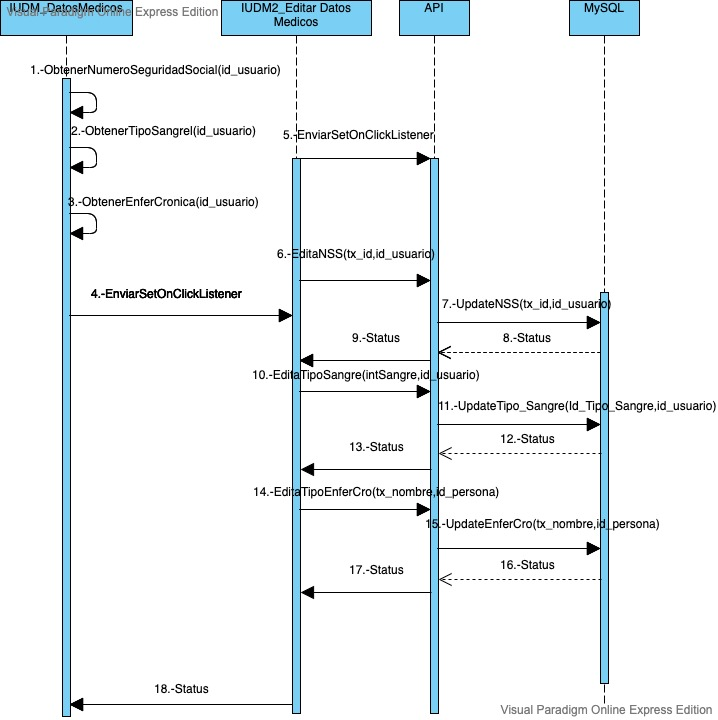
\includegraphics[width=1.0\textwidth]{AvancesPruebas/imagenes/IUDM_Datos Medicos.vpd (1)}}
	\caption{Diagrama secuencia de datos medicos}
	\label{fig:ObtenerDatosMedicos}
\end{figure}
\begin{itemize}
	\item \textbf{Envia.setOnClickListener:} La información que sera enviada en caso de querer registrar un nuevo vehiculo para un usuario.
	\item \textbf{ObtenerNumeroSeguridadSocial(id_usuario)):} Obtiene los datos correspondientes a el NSS.
	\item \textbf{ObtenerTipoSangre(id_usuario)):} Obtiene los datos correspondientes a el tipo de sangre.
	\item \textbf{ObtenerEnferCro(id_usuario)):} Obtiene los datos correspondientes a la enfermedad cronica.
	

\end{itemize}

\subsection{Edita Datos Medicos}

La figura \ref{fig:ObtenerDatosMedicos} se muestra el diagrama de secuencia correspondiente al envío de registro de un nuevo vehiculo, donde se utiliza la comunicación con la base de datos para la creación de un nuevo vehiculo.

\begin{figure}[htbp!]
	\centering
	\fbox{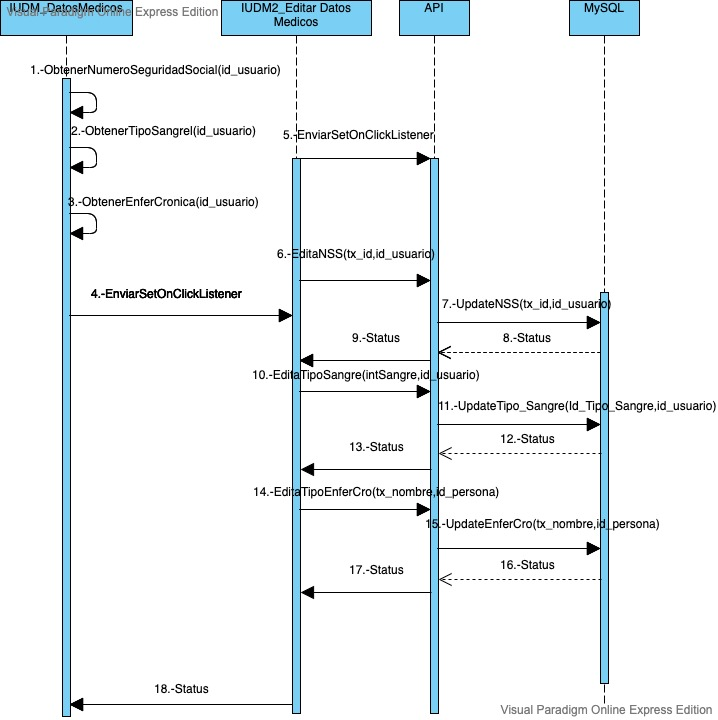
\includegraphics[width=1.0\textwidth]{AvancesPruebas/imagenes/IUDM_Datos Medicos.vpd (1)}}
	\caption{Diagrama secuencia de datos medicos}
	\label{fig:ObtenerDatosMedicos}
\end{figure}
\begin{itemize}
	\item \textbf{Envia.setOnClickListener:} La información que sera enviada en caso de querer registrar un nuevo vehiculo para un usuario.
	\item \textbf{ObtenerNumeroSeguridadSocial(id_usuario)):} Obtiene los datos correspondientes a el NSS.
	\item \textbf{ObtenerTipoSangre(id_usuario)):} Obtiene los datos correspondientes a el tipo de sangre.
	\item \textbf{ObtenerEnferCro(id_usuario)):} Obtiene los datos correspondientes a la enfermedad cronica.
	\item \textbf{ObtenerEnferCro(id_usuario)):} Obtiene los datos correspondientes a la enfermedad cronica.
	\item \textbf{Status):} Regresa el status correspondiente a el query realizado dentro de la base de datos.

	

\end{itemize}